% 2021-02-27 Banbara
%%\documentstyle[twocolumn,jsaiac]{jarticle}
%%\documentstyle[twocolumn,jsaiac]{j-article}
\documentclass[twocolumn]{jarticle}
\usepackage{jsaiac}
\usepackage [dvipdfmx]{graphicx}
\usepackage{listings}
\usepackage{plistings}
\def\lstlistingname{コード}
\usepackage{url}

\newcommand{\bhline}{\noalign{\hrule height 1.5pt}}  % 表のための太いライン

%%% For ASP
\newcommand{\asap}{\textit{teaspoon}}
\newcommand{\gringo}{\textit{gringo}}
\newcommand{\clingo}{\textit{clingo}}
\newcommand{\clasp}{\textit{clasp}}
\newcommand{\asprin}{\textit{asprin}}
\newcommand{\dlv}{\textit{DLV}}
\newcommand{\wasp}{\textit{WASP}}
\newcommand{\code}[1]{\lstinline[basicstyle=\ttfamily]{#1}}
\newcommand{\naf}[1]{\ensuremath{{\sim\!\!{#1}}}}
\newcommand{\head}[1]{\ensuremath{\mathit{head}(#1)}}
\newcommand{\body}[1]{\ensuremath{\mathit{body}(#1)}}
%\newcommand{\atom}[1]{\ensuremath{\mathit{atom}(#1)}}
\newcommand{\poslits}[1]{\ensuremath{{#1}^+}}
\newcommand{\neglits}[1]{\ensuremath{{#1}^-}}
\newcommand{\pbody}[1]{\poslits{\body{#1}}}
\newcommand{\nbody}[1]{\neglits{\body{#1}}}
%\newcommand{\Cn}[1]{\ensuremath{\mathit{Cn}(#1)}}
\newcommand{\reduct}[2]{\ensuremath{#1^{#2}}}
\newcommand{\lw}[1]{\smash{\lower1.5ex\hbox{#1}}}

\usepackage{color}

%%
\title{
\jtitle{解集合プログラミングを用いた多目的車両装備仕様問題の解法}
\etitle{Solving Multi-objective Vehicle Equipment Specification
 Problem with Answer Set Programming}
}
%%英文は以下を使用
%\title{Style file for manuscripts of JSAI 20XX}

\jaddress{竹内頼人,名古屋大学 大学院情報学研究科,住所,電話番号,Fax番号,takeuchi.raito@nagoya-u.jp}

\author{%
\jname{竹内 頼人\first}
\ename{Raito Takeuchi}
\and
\jname{田村 直之\second}
\ename{Naoyuki Tamura}
\and
\jname{番原 睦則\first}
\ename{Mutsunori Banbara}
%\and
%Given-name Surname\third{}%%英文は左を使用
}

\affiliate{
\jname{\first{}名古屋大学 大学院情報学研究科}
\ename{Graduate School of Informatics, Nagoya University}
\and
\jname{\second{}神戸大学 情報基盤センター}
\ename{Information Science and Technology Center, Kobe University}
%\and
%\third{}Affiliation \#3 in English%%英文は左を使用
}

%%
%\Vol{28}        %% <-- 28th(変更しないでください)
%\session{0A0-00}%% <-- 講演ID(必須)

\begin{abstract}
Vehicle equipment specification is, in a nutshell, 
a combination of model/grade and equipments listed in the automobile catalog.
Multi-objective Vehicle Equipment Specification Problem (MVESP) is the problem
that computes optimal vehicle equipment specifications based on trade-off 
multiple objective functions while it satisfies equipments and fuel economy 
constraints from given the number of model/grade, a set of equipment types, 
a set of equipment options and so on.
In this paper, we discuss the method to enumerate all pareto optimal answers 
of MVESP based on the fuel economy constraint called Corporate Average Fuel Economy 
(CAFE) Standards with Answer Set Programming (ASP).
In our method, the problem instance represented by Orthogonal Variability Model
(OVM) is converted to a set of facts and combined with ASP encoding 
to solve MVESP, and then we compute answers with fast ASP system.
As a result of running experiments using benchmark problems provided by a company, 
we succeeded in enumerating all pareto optimal answers for small-scale problems.

% 車両装備仕様とは,簡単に言うと,自動車のカタログに記載されている
% モデル/グレードと装備の組合せのことである.
% 多目的車両装備仕様問題は,与えられたモデル/グレードの個数,装備タイプ
% の集合,装備オプションの集合などから,装備および燃費に関する制約を満た
% しつつ,予想販売台数の最大化や装備オプション数の最小化など,トレードオ
% フの関係にある複数の目的関数のもとで最適な車両装備仕様を求める問題である.
% 本発表では,CAFE 方式と呼ばれる燃費制約に基づく多目的車両装備仕様問題
% (多目的 CAFE 問題)に対して,解集合プログラミングを用いてパレート最適解
% を列挙する方法について述べる.提案手法は,可変性モデルで表現された問題
% インスタンスを ASP のファクト形式に変換した後,それらファクトと多目的
% CAFE 問題を解くための ASP 符号化と結合し,高速 ASP システムを用いて解
% を求める.企業から提供されたベンチマーク問題を用いた実行実験の結果,小
% 規模な問題についてパレート最適解を全列挙することができた.
\end{abstract}

%\setcounter{page}{1}
\def\Style{``jsaiac.sty''}
\def\BibTeX{{\rm B\kern-.05em{\sc i\kern-.025em b}\kern-.08em%
 T\kern-.1667em\lower.7ex\hbox{E}\kern-.125emX}}
\def\JBibTeX{\leavevmode\lower .6ex\hbox{J}\kern-0.15em\BibTeX}
\def\LaTeXe{\LaTeX\kern.15em2$_{\textstyle\varepsilon}$}


\begin{document}
\maketitle


\section{はじめに}\label{sec:introduction}
% ------------------------------------------
\begin{figure*}[t]
  \centering
  \thicklines
  \setlength{\unitlength}{1.28pt}
  \small
  \begin{picture}(280,57)(4,-10)
    \put( -35, 20){\dashbox(70,24){\shortstack{組合せ最適化問題\\のインスタンス}}}
    \put( 45, 20){\framebox(50,24){変換器}}
    \put(105, 20){\dashbox(70,24){\shortstack{ASPファクト}}}
    \put(105,-10){\dashbox(70,24){\shortstack{ASP符号化\\(論理プログラム)}}}
    \put(185,-10){\framebox(60,54){}}
    \put(189, 25){\framebox(52,12){ASPソルバー}}
    \put(190, -5){\framebox(50,12){LNPS}}
    % \put(180, 20){\framebox(50,24){ASPシステム}}
    \put(255, 20){\dashbox(70,24){\shortstack{組合せ最適化問題\\の最適解}}}
    \put(  35, 32){\vector(1,0){10}}
    \put(  95, 32){\vector(1,0){10}}
    \put(175, 32){\vector(1,0){10}}
    \put(245, 32){\vector(1,0){10}}
    \put(175, +2){\line(1,0){4}}
    \put(179, +2){\line(0,1){30}}
    \put(205,  7){\vector(0,1){17}}
    \put(225, 24){\vector(0,-1){17}}
    \put(190, 48){提案ソルバー}
  \end{picture}  
\caption{提案ソルバー\textit{asprior}の構成}
\label{fig:arch}
\end{figure*}

%%% Local Variables: 
%%% mode: latex
%%% TeX-master: "paper"
%%% End: 

% ------------------------------------------

\textbf{車両装備仕様}とは,簡単に言うと,自動車のカタログに記載されて
いる車種(モデルやグレード)と装備の組合せのことである.
車両装備仕様を決めるには,販売される国や地域の法規や規制,
地域や市場の特性,市場の嗜好や競合など十分に考慮する必要がある.
しかし,現状では専門知識をもつ技術者の多大な労力が費やされている.
そのため,車両装備仕様の自動生成は自動車メーカーにとって重要な課題の一
つである.

\textbf{企業平均燃費}
(Corporate Average Fuel Efficiency; CAFE
\cite{mlit18:cafe})
は自動車の燃費規制で,車種別ではなくメーカー全体での出荷
台数を加味した平均燃費を算出し,規制をかける方式である.
この方式の特長は,ある車種では燃費基準を達成できなくても,
他の車種の燃費を向上させることで基準を達成できることが可能な点である.
このCAFE方式は,欧米で採用され,日本でも2020年度から導入されている.

\textbf{多目的車両装備仕様問題}
(Multi-objective Vehicle Equipment Specification Problem)
は,与えられた車種の数,
装備タイプの集合,
装備オプションの集合から,
装備および燃費に関する制約を満たしつつ,
予想販売台数の最大化や装備オプション数の最小化など,トレードオフの関係にある
複数の目的関数のもとで最適な車両装備仕様を求める組合せ最適化問題の一種である.
本論文では,CAFE 方式に基づく多目的車両装備仕様問題
(以降,\textbf{多目的CAFE問題}と呼ぶ)を対象とする.

\textbf{解集合プログラミング}
(Answer Set Programming; ASP
\cite{Gelfond88:iclp,Inoue08:jssst})
は,論理プログラミングから派生した宣言的プログラミングパラダイムである.
ASP言語は一階論理に基づく知識表現言語の一種である.
論理プログラムは ASP のルールの有限集合である.
ASPシステムは論理プログラムから安定モデル意味論~\cite{Gelfond88:iclp}
に基づく解集合を計算するシステムである.
近年,SAT 技術を応用した高速 ASP システムが実現され,
システム検証,システム生物学,プランニングなど様々な分野への実用的応用
が急速に拡大している~\cite{Erdem16:ai-magazine}.

本論文では,ASP に基づく多目的 CAFE 問題ソルバーの実装と評価ついて述べる.
提案ソルバーは,可変性モデルで表現された問題インスタンスを ASP のファ
クト形式に変換した後,それらファクトと多目的 CAFE 問題を解くための ASP
符号化と結合し,高速 ASP システムを用いて
パレート最適解を列挙する(図~\ref{fig:arch}参照).
%
考案した ASP 符号化は,多目的 CAFE 問題の制約と2つの目的関数を簡潔に表
現できる.この符号化は,単目的 CAFE 問題の ASP 符号化~\cite{Takeuchi20:jssst}
の自然な拡張になっている.
%
ASP システムとしては,{\asprin}システム~\cite{Brewka15:casp}を使用する.
{\asprin}は,広く普及している{\clingo}をベースに,
多目的最適化や解集合の間の選好順序を記述できるように拡張されたシステム
である.
%
企業から提供を受けた小規模・中規模の多目的 CAFE 問題に対して実行実験を
行った結果,小規模な問題のパレート最適解を全列挙をすることができた.

%%% Local Variables:
%%% mode: latex
%%% TeX-master: "paper"
%%% End:

\section{多目的CAFE問題}\label{sec:background}

%-------------------------------------------------------
\begin{figure*}[t]\centering
  \begin{minipage}[b]{0.5\linewidth}
    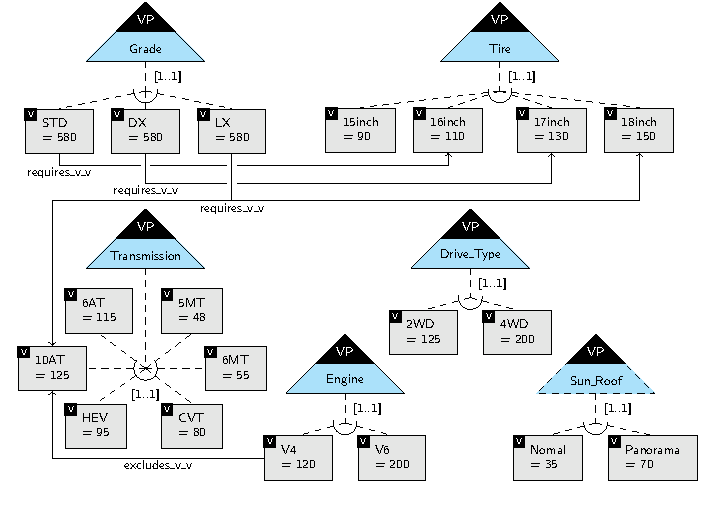
\includegraphics[width=1.0\linewidth]{images/ovm_example.pdf}
    \caption{CAFE問題の例}\label{fig:ovm}
  \end{minipage}\hfill
  \begin{minipage}[b]{0.4\linewidth}
    \begin{tabular}{l|c|c|c}\hline\hline
      & 車種1  & 車種2  & 車種3\\\hline
      \textsf{Grade}        & \textsf{STD}    & \textsf{DX}     & \textsf{LX}\\
      \textsf{Drive\_Type}  & \textsf{2WD}    & \textsf{2WD}    & \textsf{4WD}\\
      \textsf{Engine}	    & \textsf{V6}     & \textsf{V6}     & \textsf{V6}\\
      \textsf{Tire}	    & \textsf{16inch} & \textsf{17inch} & \textsf{18inch}\\
      \textsf{Transmission} & \textsf{6AT}    & \textsf{HEV}    & \textsf{10AT}\\
      \textsf{Sun\_Roof}    & -               & -               & -  \\\hline\hline
      IWR 値の総和           & 1,130  & 1,130   & 1,255 \\ %\hline
      燃費(km/L)      & 8.8  & 8.8     & 8.0 \\ %\hline
      予想販売台数    & 2,007   & 2,007   & 1,511  \\ \hline
      平均燃費(km/L)  & \multicolumn{3}{c}{8.5} \\ 
      予想販売台数(合計)  & \multicolumn{3}{c}{5,525} \\ 
      装備オプション数 & \multicolumn{3}{c}{12}	\\ \hline
    \end{tabular}
    \caption{CAFE 問題の解}\label{fig:ovm:ans}
\end{minipage}
\end{figure*}
%-------------------------------------------------------

図~\ref{fig:ovm}に CAFE 問題の例を示す.
この例は,ソフトウェアプロダクトライン開発の分野で用いられる
\textbf{可変性モデル} (Orthogonal Variability Model; OVM~\cite{Pohl05:sple})
によって記述されている.
%
\textsf{VP}でタグ付けされた三角形は,車種ごとに選択されるオプショ
ンが変わりうる\textbf{装備タイプ}を表す.
装備タイプの具体的な\textbf{装備オプション}は,
\textsf{V}でタグ付けされた長方形で表される.
長方形の中の数値は,IWR (Inertial Working Rating) と呼ばれ,
直観的には各装備オプションの重量を表す.
装備タイプと装備オプションの対応関係は,選択肢(破線)と
多重度($[lb..ub]$)で表される.
多重度の$lb$と$ub$は,それぞれ,各装備タイプで選択可能な装備オプション
数の上限値と下限値である.
装備タイプ同士,装備オプション同士,および,装備タイプと装備オプション
の間の依存関係は,実線矢印で表され,要求(\textsf{requires})と排他
(\textsf{excludes})の2種類がある.
%
図~\ref{fig:ovm}の問題例は,
6個のタイプ,19個のオプション,5個の依存関係から構成される.
各装備タイプの選択可能な装備オプション数はすべて1である.
例えば,
装備タイプ\textsf{Transmission}は,6つの装備オプション
\textsf{6AT},
\textsf{10AT},
\textsf{HEV},
\textsf{CVT},
\textsf{6MT},
\textsf{5MT}
からちょうど1つを選択可能である.また,
\textsf{10AT}と\textsf{V4}は,排他的な依存関係にある.
%
本論文では,
各車種に対して必須な装備タイプは実線のノードで表し,
\textsf{Sun\_Roof}のような必須でないものは破線のノードで表す.

車種数を$n$,
CAFE 基準値を$t$としたとき,
CAFE 問題の制約は以下の通りである.
\begin{description}
\item[範囲制約]: 各車種について,各装備タイプで選択される装備オプショ
    ン数は,与えられた上下限値の範囲内でなければならない.
\item[依存制約]: 各車種について,与えられた依存関係を満たさなければならない.
\item[燃費制約]: 車種$g\ (1\leq g\leq n)$の
  燃費と予想販売台数をそれぞれ$FE_{g}$と$SV_{g}$とするとき,
  以下の CAFE 規制を満たさなければならない.
\vskip -1em	  
  \[\begin{array}{lcr}
      & & \\
      \displaystyle\frac{\sum_{g=1}^{n} FE_{g}\cdot SV_{g}}{\sum_{g=1}^{n} SV_{g}}
      &
        \geq 
      &
        t \\
      & & 
   \end{array}\]
  不等式の左辺は,$n$車種の\textbf{平均燃費}を表している.
  $FE_{g}$と$SV_{g}$は,車種$g$におけるIWR値の総和から,
  企業が独自に保有する燃費テーブルと販売台数テーブルを基に計算される.
\end{description}

CAFE 問題の目的関数は,以下の通りである.
\begin{description}
 \item[予想販売台数の最大化]: 各車種ごとに求められる予想販売台数の合計を最大化する.
 \item[装備オプション数の最小化]: $n$車種全体で,使用される装備オプションの数を最小化する.
   これは,製造ラインの削減や,大量生産を促進することを狙いとしている.
\end{description}

本論文で対象とする多目的 CAFE 問題は,
与えられた問題インスタンス(可変性モデルで表現),
車種数$n$,
CAFE 基準値$t$,
燃費テーブルと販売台数テーブルから,
範囲制約,依存制約,燃費制約を満たしつつ,
予想販売台数の最大化と装備オプション数の最小化の2つの目的関数のもとで,
パレート最適解を求める問題である.

図~\ref{fig:ovm:ans}に,
問題インスタンス (図~\ref{fig:ovm}),
車種数$n=3$,
CAFE 基準値$t=8.5$に対する
実行可能解の一例を示す.
各車種の燃費は,左から順に 8.8, 8.8, 8.0km/L となり,
車種3は CAFE 基準値を満たしていないないが,
3台の平均燃費は 8.581km/L となり,CAFE 規制を満たしている.

%%% Local Variables:
%%% mode: latex
%%% TeX-master: "paper"
%%% End:

\section{多目的CAFE問題のASP符号化}\label{sec:proposal}

ASPの言語は,
一般拡張選言プログラム
(General Extended Disjunctive Program)
をベースとしている\cite{Inoue08:jssst}.
本節では,説明の簡略化のため,そのサブクラスである
標準論理プログラムについて説明する.
以降,標準論理プログラムを単に{\bf 論理プログラム}と呼ぶ.

論理プログラムは,以下の形式の\textbf{ルール}の有限集合である.
\begin{equation}
  \label{eq:rule}
  a_0\leftarrow a_1,\dots,a_m,\naf{a_{m+1}},\dots,\naf{a_n}
\end{equation}
このルールの直観的な意味は,
「$a_1,\ldots,a_m$がすべて成り立ち,$a_{m+1},\ldots,a_n$のそれぞれが成
り立たないならば,$a_0$が成り立つ」である.
ここで,
$0\leq m\leq n$ であり,
各$a_i$はアトム,
$\naf{}$は\textbf{デフォルトの否定}
\footnote{\textbf{失敗による否定}とも呼ばれる.述語論理で定義される否定($\neg$)とは意味が異なる.},
``$,$''は連言を表す.
$\leftarrow$の左側を\textbf{ヘッド},右側を\textbf{ボディ}と呼ぶ.
ボディが空のルール(すなわち\(a_0\leftarrow\))を\textbf{ファクト}と呼び,
$\leftarrow$を省略してよい.

ヘッドが空のルールを\textbf{一貫性制約}と呼び,以下のように表す.
\begin{equation}
  \label{eq:constr}
  \leftarrow a_1,\dots,a_m,\naf{a_{m+1}},\dots,\naf{a_n}
\end{equation}
例えば,一貫性制約
``\(\leftarrow a_1,a_2\)''は,「$a_1$と$a_2$が両方同時に成り立つことはない」を意味し,
``\(\leftarrow a_1, \naf{a_{2}}\)''は,「$a_1$が成り立つならば,$a_2$が成り立つ」を意味する.

ASP言語には,組合せ問題を簡潔に記述するために,
\textbf{アグリゲート}(aggregate)と呼ばれる拡張構文がいくつか用意されている.
例えば,\textbf{選択子}``$\{a_1;\ldots;a_n\}$.''は,
アトム集合\(\{a_1,\ldots,a_n\}\)の任意の部分集合を解集合に含めることを意味する.
\textbf{個数制約}は選択子の両端に選択可能な個数の上下限を付けたものである.
例えば,``\(lb\ \{a_1;\dots;a_n\}\ ub \leftarrow Body\)''と書くと,
「$Body$が成り立つならば,$a_1,\dots,a_n$のうち,$lb$個以上$ub$個以下
が成り立つ」を意味する.
\textbf{重み付き個数制約}``\(t = \#sum\ \{w_1:a_1;\ldots;w_n:a_n\}\).''は,
$a_1,\dots,a_n$のうち真となるアトムの重み和が項$t$に等しくなることを意味する.
項$w_i$は重みを表し,演算子としては``=''以外にも``$\leq$'',``$\geq$''などを使用できる.
さらに,重み付き個数制約の``$\#sum$''を,``$\#max$''や``$\#min$''に書
き換えると,重み和ではなく,真となるアトムの重みの最大値や最小値を求め
ることができる.

近年,
{\clingo}~\footnote{\url{https://potassco.org/}},
{\dlv}~\footnote{\url{http://www.dlvsystem.com/dlv/}},
{\wasp}~\footnote{\url{https://www.mat.unical.it/ricca/wasp/}}
など,SATソルバー技術を応用した高速なASPシステムが開発されている.
なかでも{\clingo}は,高性能かつ高機能なASPシステムとして世界中で広く使われている.
これらの高速ASPシステムは,変数を含む論理プログラムを変数を含まない論
理プログラムに変換(\textbf{基礎化})したのち,ASPソルバーを用いて解集合を計算する.
本論文で使用するASPシステム{\clingo}は,基礎化のためのグラウンダー
{\gringo}とASPソルバー{\clasp}をシームレスに結合したものである.

本論文では,論理プログラムの解集合の中で,選好関係の宣言・評価を可能にするシステム
{\asprin}~\cite{Brewka15:casp}も使用する.
選好関係は,{\bf 選好文}と呼ばれるプログラムの中で,次のように宣言される.
\begin{equation}
  \label{eq:preference}
  \#preference(s,t)\{e_1,\dots,e_n\}
\end{equation}
ここで,$s$ と $t$ はそれぞれ選好の名称とタイプであり,
引数の各 $e_j$ は選好の要素である. 
{\asprin} では,新たに選好タイプを定義することも可能だが,
いくつかの選好タイプはあらかじめライブラリに定義されており,
それを利用することで簡潔に選好関係を記述することができる.
% 本発表では選好のタイプとして$less(weight), more(weight), pareto$ を使用する.
そして,次のように最適化命令を記述することで,選好関係 $s$ について
最適な解集合を得ることができる.
\begin{equation}
 \label{eq:optimize}
 \#optimize(s)
\end{equation} 
このとき,{\asprin}では繰り返しASPソルバーを呼び出すことで,
最適な解集合を段階的に計算する.

本論文で提案する多目的CAFE問題の解法では,
与えられた問題インスタンスをASPのファクト形式に変換した後,
それらファクトと多目的CAFE問題を解くためのASP符号化(論理プログラム)を結合した上で,
高速ASPシステム{\clingo}と{\asprin}を用いて解を求める(図\ref{fig:arch}参照).
本論文では,説明の簡略化のため,各タイプが選択可能なオプション数の上下限値を1とする.

多目的CAFE問題の問題インスタンスは,CAFE基準値を除いてアトムに変換され,
ファクトとして表現される.
CAFE基準値はASPの定数$t$で表すものとし,実行時に\clingo のオプションから値を指定する.
各アトムは,表\ref{tab:fact}のように第\ref{sec:background}節の各入力に対応する.
\begin{table}[t]
 \caption{問題インスタンスのアトム}
 \centering
 \tabcolsep = 1mm
 \begin{tabular}{ll} \bhline
  アトム & 対応する入力番号 \\ \hline
  $vp\_def(vp)$ & 入力\ref{input:vp} \\
  $v\_def(v,vp,x)$ & 入力\ref{input:v}, \ref{input:vp-v}, \ref{input:iwr} \\
  $require\_vp(vp)$ & 入力\ref{input:req_vp} \\
  $require\_v\_v(v_1,v_2)$ & 入力\ref{input:dependency} \\
  $exclude\_v\_v(v_1,v_2)$ & 入力\ref{input:dependency} \\
  $group(1..n)$ & 入力\ref{input:g} \\ 
  $require\_g\_v(i,v)$ & 入力\ref{input:init} \\
  $fe\_map(s,fe)$ & 入力\ref{input:fe} \\
  $sv\_map(s,fe)$ & 入力\ref{input:sv} \\ \hline
 \end{tabular}
 \label{tab:fact}
\end{table}

多目的CAFE問題の各制約は,ASPの個数制約および一貫性制約を使用して
簡潔に表現される(コード\ref{code:basic.lp}).
また,コード\ref{code:basic.lp}の8〜12行目では,
各タイプが選択可能なオプション数の上下限値,および,必須かどうかの別を考慮することで,
IWR値の和である\code{S}の上下限をより厳密に計算するように工夫がされている.
これにより,\code{iwr(S,G)}に関する基礎化後のルール数を少なく抑えることができる.

%----------------------------------------
\lstinputlisting[float=tb,caption={%
  制約の符号化},%
captionpos=b,frame=single,label=code:basic.lp,%
numbers=left,%
breaklines=true,%
columns=fullflexible,keepspaces=true,%
xrightmargin=1zw,% 
xleftmargin=1zw,% 
basicstyle=\ttfamily\footnotesize]{codes/basic.lp} 
%----------------------------------------


多目的CAFE問題の選好文は,コード\ref{code:preference.lp}のように定義される.
目的関数である予想販売台数の最大化とオプション数の最小化は,
それぞれ選好名\code{max\_sv}, \code{min\_op} として定義している.
9行目で使用している選好タイプ\code{pareto} は,
選好文中で定義された選好名を引数に取り,
それらの選好関係についてパレートな解を得ることができる.
すなわち,解集合$S_1$が$S_2$よりも厳密に好まれるならば,かつそのときに限り,
引数のすべての選好関係に関して,少なくとも$S_1$は$S_2$と同等で,かつ,
少なくとも1つの選好関係に関して$S_1$は$S_2$より厳密に優れている.

%----------------------------------------
\lstinputlisting[float=tb,caption={%
  選好文},%
captionpos=b,frame=single,label=code:preference.lp,%
numbers=left,%
breaklines=true,%
columns=fullflexible,keepspaces=true,%
xrightmargin=1zw,% 
xleftmargin=1zw,% 
basicstyle=\ttfamily]{codes/preference.lp} 
%----------------------------------------

第\ref{sec:background}節と同様に多目的CAFE問題の例
(図\ref{fig:ovm_example})を用いて,
最適解をすべて列挙した結果を表~\ref{tab:prt_ans}に示す.
予想販売台数とオプション数の値から,
得られた各装備仕様が互いにトレードオフの関係にあることが分かる.
本解法の利点は,このような定性的に得られた複数の解を人が見比べることで,
定量的な判断により最終的な決定をすることができる点である.

%----------------------------------------
\begin{table*}[t]
   \centering
 % \small
 \tabcolsep=1mm
  \caption{CAFE問題(図~\ref{fig:ovm_example})のパレート解}
  \begin{tabular}{l|l|c|c|c||c|c|c||c|c|c||c|c|c} \bhline
   \multicolumn{2}{l|}{} & \multicolumn{3}{c||}{解1} & \multicolumn{3}{c||}{解2} & \multicolumn{3}{c||}{解3} & \multicolumn{3}{c}{解4}\\ \hline
   \multicolumn{2}{l|}{装備仕様} & 1 & 2 & 3 & 1 & 2 & 3 & 1 & 2 & 3 & 1 & 2 & 3 \\ \hline
   装備 & \textsf{Grade} & \textsf{STD} & \textsf{DX} & \textsf{LX} & \textsf{STD} & \textsf{DX} & \textsf{LX} & \textsf{STD} & \textsf{DX} & \textsf{LX} & \textsf{STD} & \textsf{DX} & \textsf{LX} \\
       & \textsf{Drive\_Type} & \textsf{2WD} & \textsf{2WD} & \textsf{4WD} & \textsf{2WD} & \textsf{2WD} & \textsf{4WD} & \textsf{2WD} & \textsf{2WD} & \textsf{2WD} & \textsf{2WD} & \textsf{2WD} & \textsf{2WD} \\
       & \textsf{Engine} & \textsf{V6} & \textsf{V6} & \textsf{V6} & \textsf{V6} & \textsf{V6} & \textsf{V6} & \textsf{V6} & \textsf{V6} & \textsf{V6} & \textsf{V6} & \textsf{V6} & \textsf{V6} \\
       & \textsf{Tire} & \textsf{16inch} & \textsf{17inch} & \textsf{18inch} & \textsf{16inch} & \textsf{17inch} & \textsf{18inch} & \textsf{16inch} & \textsf{17inch} & \textsf{18inch} & \textsf{16inch} & \textsf{17inch} & \textsf{18inch} \\
       & \textsf{Transmission} & \textsf{6AT} & \textsf{HEV} & \textsf{10AT} & \textsf{10AT} & \textsf{HEV} & \textsf{10AT} & \textsf{10AT} & \textsf{HEV} & \textsf{10AT} & \textsf{10AT} & \textsf{10AT} & \textsf{10AT} \\
       & \textsf{Sun\_Roof} & \textsf{-} & \textsf{-} & \textsf{-} & \textsf{-} & \textsf{-} & \textsf{-} & \textsf{-} & \textsf{-} & \textsf{-} & \textsf{-} & \textsf{-} & \textsf{-} \\ \hline
   \multicolumn{2}{l|}{予想販売台数(合計)}  & \multicolumn{3}{c||}{\bf 5,525} & \multicolumn{3}{c||}{\bf 5,475} & \multicolumn{3}{c||}{\bf 5,135} & \multicolumn{3}{c}{\bf 4,723} \\ 
   \multicolumn{2}{l|}{オプション数} & \multicolumn{3}{c||}{\bf 12} & \multicolumn{3}{c||}{\bf 11} & \multicolumn{3}{c||}{\bf 10} & \multicolumn{3}{c}{\bf 9} \\ \hline
   %\multicolumn{14}{c}{}
  \end{tabular}
 \label{tab:prt_ans}
\end{table*}
%----------------------------------------
\section{実行実験}
%----------------------------------------------
\begin{table}[t]\centering
  \caption{ベンチマーク問題}
  \vskip 1em
  % \renewcommand{\arraystretch}{0.9}
  % \tabcolsep = 0.9mm
  \begin{tabular}{lrrrr}\hline
    問題名 & \#装備タイプ	& \#装備オプション	& \#依存制約 	\\\hline
    small   & 8		& 21	& 4	  	        \\
    medium  & 86	& 229	& 147	  	        \\
    big	    & 315	& 1,337	& 0	          	\\\hline
    & & & \\
  \end{tabular}
 \label{tab:bench}
\end{table}
%----------------------------------------------

%----------------------------------------------
\begin{table}[t]\centering
  \caption{実験結果: CPU時間}
  \vskip 1em  
  % \renewcommand{\arraystretch}{0.9}
  % \tabcolsep = 0.9mm
  \begin{tabular}{cr|rr}\hline
    \lw{問題名} & CAFE & パレート   & \lw{CPU時間(秒)} \\
           & 基準値$t$ & 最適解の数 &  \\ \hline
    small  & 8.5   & 8*      &   35.136     \\
    small  & 9.0   & 5*      & 1085.354     \\
    small  & 9.5   & --       & $timeout$    \\
    small  & 10.0  & 1*      &    1.863     \\
    small  & 10.5  & 0*      &    0.221     \\\hline
  \end{tabular}
  \label{tab:result}
\end{table}
%----------------------------------------------

提案ソルバーの有効性を評価するために,多目的 CAFE 問題のパレート
最適解を全列挙する実行実験を行った.
ベンチマーク問題には,企業から提供を受けた3問を使用した(表~\ref{tab:bench}参照).
small は小規模な問題,
medium は現実規模の問題,
big は大規模な問題である.
各問題に対して,
5種類の CAFE 基準値$t = 8.5, 9.0, 9.5, 10.0, 10.5$km/Lを適用し,
計15問に対して実験を行なった.車種の数は$n=3$とした.
ASPシステムには{\asprin}-3.1.1を利用し,
1問あたりの制限時間は3時間とした.
実験環境は,Mac OS, 3.2GHz Intel Core i7, 64GB メモリである.

表~\ref{tab:result}に小規模な問題smallの実験結果を示す.
左の列から順に,問題名,CAFE基準値$t$,得られたパレート最適解の数,
解の全列挙に要した CPU 時間となっている.
記号`$\ast$'は,パレート最適解の全列挙に成功したことを意味する.
逆に,記号`--'は,パレート最適解が一つも得られなかったことを意味する.
%
実験の結果,5問中3問に対して,パレート最適解を全列挙することができた.
また,$t=10.5$の場合のパレート最適解の数は0であり,実行可能解が存在し
ないことが確認できた.
medium と big については,実行可能解は得られたものの,パレート最適解を
得ることはできなかった.

%%% Local Variables:
%%% mode: japanese-latex
%%% TeX-master: "paper"
%%% End:

\section{おわりに}

本論文では,ASP に基づく多目的 CAFE 問題ソルバーの実装と評価ついて述べた.
ASP 言語の表現力の高さを活かし,
多目的 CAFE 問題の制約と目的関数を簡潔に表現できることを確認した.
企業から提供を受けたベンチマーク問題を用いて評価実験を行った結果,
小規模な問題に対して,パレート最適解を全列挙をすることができた.

%%%%%%%%%%%%%%%%%%%%%%%%%%%%%%%%%%%%%%%%%%%%%%%%%%%
\vskip 1em
\begin{itemize}\Large
\item 関連研究(TODO)
\item 参考文献追加(TODO)
\item 今後の課題(TODO)
\end{itemize}
%%%%%%%%%%%%%%%%%%%%%%%%%%%%%%%%%%%%%%%%%%%%%%%%%%%


%%% Local Variables:
%%% mode: latex
%%% TeX-master: "paper"
%%% End:


\bibliographystyle{jsai}
\bibliography{jsai2021}
\end{document}

%%% Local Variables:
%%% mode: japanese-latex
%%% TeX-master: t
%%% End:
